\documentclass[11pt,letterpaper]{article}
\usepackage[utf8]{inputenc}
\usepackage[T1]{fontenc}
\usepackage{amsmath,amssymb}
\usepackage{geometry}
\usepackage{xcolor}
\usepackage{tikz}
\usetikzlibrary{shapes.geometric, arrows.meta, positioning, decorations.pathreplacing}
\usepackage{tcolorbox}
\usepackage{enumitem}
\usepackage{fancyhdr}
\usepackage{booktabs}
\usepackage{hyperref}
\usepackage{array}

\geometry{margin=0.9in}

\definecolor{asumaroon}{RGB}{140,29,64}
\definecolor{darkblue}{RGB}{31,78,121}
\definecolor{lightblue}{RGB}{213,232,240}
\definecolor{lightgray}{RGB}{245,245,245}
\definecolor{vmgreen}{RGB}{119,185,0}
\definecolor{checkgreen}{RGB}{0,128,0}

\pagestyle{fancy}
\fancyhf{}
\fancyhead[L]{\small CEE 412/598 Transportation Systems}
\fancyhead[R]{\small GTFS2GMNS Reading \& Concepts}
\fancyfoot[C]{\thepage}

\tcbuselibrary{skins,breakable}
\newtcolorbox{readingbox}[1]{colback=vmgreen!8, colframe=vmgreen!70!black, fonttitle=\bfseries, title=#1, breakable}
\newtcolorbox{questionbox}[1]{colback=lightblue, colframe=darkblue, fonttitle=\bfseries, title=#1, breakable}
\newtcolorbox{conceptbox}[1]{colback=lightgray, colframe=asumaroon, fonttitle=\bfseries, title=#1, breakable}
\newtcolorbox{connectionbox}[1]{colback=yellow!10, colframe=orange!70!black, fonttitle=\bfseries, title=#1, breakable}

\newcommand{\cmark}{$\square$\hspace{0.3em}}
\newcommand{\fillin}{\underline{\hspace{2cm}}}

\begin{document}

\begin{center}
{\LARGE\bfseries\color{asumaroon} GTFS2GMNS: Reading \& Concept Checklist}\\[0.3cm]
{\large Ensuring You Understand Before You Compute}\\[0.3cm]
\end{center}

\begin{conceptbox}{Core Principle}
\textbf{GTFS files are not static data---they are decision variables.}\\[0.2cm]
\texttt{stops.txt} $\rightarrow$ Where should we place stops? (coverage vs. speed)\\
\texttt{stop\_times.txt} $\rightarrow$ How often should buses run? (frequency vs. fleet cost)\\
\texttt{routes.txt} $\rightarrow$ Which corridors should we serve? (demand vs. equity)
\end{conceptbox}

%===========================================
\section{Reading 1: Valley Metro Service Planning (Lecture 2.1)}
%===========================================

\begin{readingbox}{Document: Joe Gregory's Presentation (27 slides)}
\textbf{Who:} Joe Gregory, Manager of Service Planning \& GIS, Valley Metro\\
\textbf{Focus:} Real-world transit planning in Phoenix metropolitan area
\end{readingbox}

\subsection*{Reading Checklist}

\cmark Read slides 1--7: System perspectives (Riders, Operators, Funders)

\cmark Read slides 8--12: Origin-Destination Study methodology

\cmark Read slides 13--16: \textbf{Fiesta BUZZ Case Study} (critical!)

\cmark Read slides 17--21: Autonomous Vehicle Pilot integration

\cmark Read slides 22--27: Human Spectrogram discussion questions

\subsection*{Concept Verification Questions}

\begin{questionbox}{Questions from Lecture 2.1 (Fill in or answer briefly)}

\textbf{Q1.} The Valley Metro O-D study collects \fillin completed surveys every 3--5 years.
\vspace{0.2cm}

\textbf{Q2.} In the Fiesta BUZZ case (slide 14), the round-trip runtime was \fillin minutes, and On-Time Performance suffered because drivers lacked sufficient \fillin time.
\vspace{0.2cm}

\textbf{Q3.} The solution (slide 16) involved three changes: (a) \fillin routes, (b) add \fillin vehicle(s), and (c) adjust \fillin locations.
\vspace{0.2cm}

\textbf{Q4.} Why does ``interlining'' (connecting DBUZ and FBUZ) help reduce fleet requirements?\\[1cm]

\textbf{Q5.} From slide 25, should transit be run more like a social service or a business? What's your view and why? (2 sentences)\\[1.5cm]

\end{questionbox}

%===========================================
\section{Reading 2: Bus and Driver Scheduling (Lecture 2.2)}
%===========================================

\begin{readingbox}{Document: Scheduling Overview (PowerPoint)}
\textbf{Focus:} The mathematics connecting timetables to fleet size and crew requirements
\end{readingbox}

\subsection*{Reading Checklist}

\cmark Understand the definition of \textbf{cycle time} (round-trip including layovers)

\cmark Understand the definition of \textbf{deadhead} (non-revenue vehicle movement)

\cmark Understand the definition of \textbf{blocking} (assigning trips to vehicles)

\cmark Memorize the fleet equation: $N = T_{\text{cycle}} / h$

\subsection*{Concept Verification Questions}

\begin{questionbox}{Questions from Lecture 2.2 (Calculate or explain)}

\textbf{Q6.} Write the fleet equation: $N_{\text{vehicles}} = $ \fillin

\vspace{0.2cm}
\textbf{Q7.} If cycle time = 60 min and headway = 10 min, how many vehicles are needed? \fillin

\vspace{0.2cm}
\textbf{Q8.} If you want to \textbf{double} frequency (halve headway), what happens to fleet size? \fillin

\vspace{0.2cm}
\textbf{Q9.} Define ``deadhead'' in one sentence:\\[0.8cm]

\textbf{Q10.} Why is minimizing deadhead important for transit agencies? (cost perspective)\\[1cm]

\end{questionbox}

%===========================================
\section{Reading 3: GTFS2GMNS User Guide (Lecture 2.4)}
%===========================================

\begin{readingbox}{Document: Technical User Guide (15 pages)}
\textbf{Source:} ASU Trans+AI Lab\\
\textbf{Focus:} Converting GTFS to network format for modeling and optimization
\end{readingbox}

\subsection*{Reading Checklist}

\cmark Read Section 1: Overview (what GTFS2GMNS does)

\cmark Read Section 2: Data flow structure (Figure 1 is essential!)

\cmark Read Section 4: Illustrative Example (two-layer network)

\cmark Read Section 5: BART case study

\cmark Read Section 6.1--6.4: Applications (Assignment, Accessibility, Equity)

\cmark Read Section 6.5: Linear Programming formulations

\subsection*{Concept Verification Questions}

\begin{questionbox}{Questions from Lecture 2.4 (Identify and explain)}

\textbf{Q11.} GTFS2GMNS produces two output files: \texttt{\fillin} and \texttt{\fillin}

\vspace{0.2cm}
\textbf{Q12.} List the \textbf{four types of nodes}:
\begin{enumerate}[nosep]
    \item Physical nodes (stops/stations)
    \item \fillin nodes
\end{enumerate}

\vspace{0.2cm}
\textbf{Q13.} List the \textbf{four types of links}:
\begin{enumerate}[nosep]
    \item Service links (connect stops along routes)
    \item \fillin links (passenger boards)
    \item \fillin links (passenger alights)  
    \item \fillin links (walk between stops)
\end{enumerate}

\vspace{0.2cm}
\textbf{Q14.} In the BART example (Section 5.3.1), how many physical stations? \fillin \quad Routes? \fillin

\vspace{0.2cm}
\textbf{Q15.} What field in \texttt{link.csv} contains travel time? \texttt{\fillin}

\vspace{0.2cm}
\textbf{Q16.} What field in \texttt{link.csv} contains vehicle/link capacity? \texttt{\fillin}

\vspace{0.2cm}
\textbf{Q17.} From Section 6.5, the transit assignment LP minimizes total \fillin subject to flow conservation and \fillin constraints.

\end{questionbox}

%===========================================
\section{The Four-Layer Framework}
%===========================================

\begin{conceptbox}{Understanding the Layers}
\begin{center}
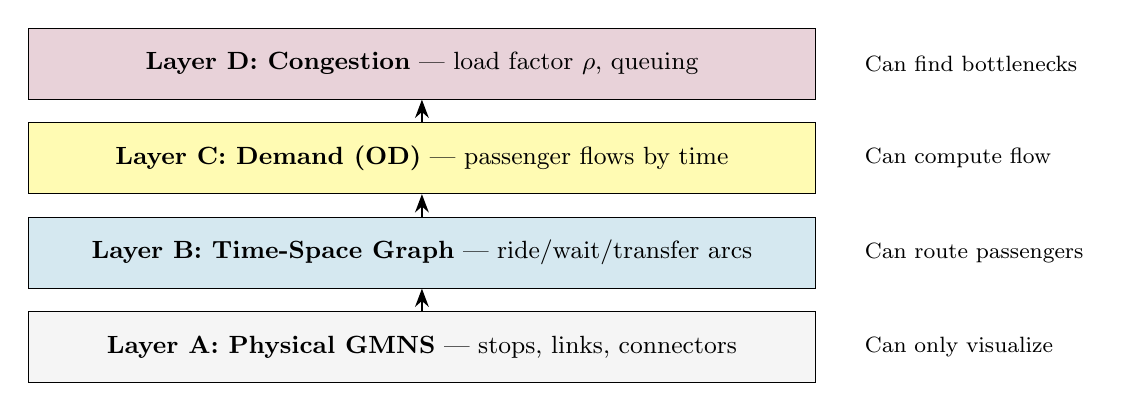
\begin{tikzpicture}[
    layer/.style={rectangle, draw, minimum width=10cm, minimum height=0.9cm, align=center, font=\small},
    arrow/.style={-Stealth, thick}
]
\node[layer, fill=lightgray] (A) at (0,0) {\textbf{Layer A: Physical GMNS} --- stops, links, connectors};
\node[layer, fill=lightblue] (B) at (0,1.2) {\textbf{Layer B: Time-Space Graph} --- ride/wait/transfer arcs};
\node[layer, fill=yellow!30] (C) at (0,2.4) {\textbf{Layer C: Demand (OD)} --- passenger flows by time};
\node[layer, fill=asumaroon!20] (D) at (0,3.6) {\textbf{Layer D: Congestion} --- load factor $\rho$, queuing};

\draw[arrow] (A) -- (B);
\draw[arrow] (B) -- (C);
\draw[arrow] (C) -- (D);

\node[right, font=\footnotesize] at (5.5,0) {Can only visualize};
\node[right, font=\footnotesize] at (5.5,1.2) {Can route passengers};
\node[right, font=\footnotesize] at (5.5,2.4) {Can compute flow};
\node[right, font=\footnotesize] at (5.5,3.6) {Can find bottlenecks};
\end{tikzpicture}
\end{center}
\end{conceptbox}

\begin{questionbox}{Layer Understanding Check}

\textbf{Q18.} If you only have Layer A (node.csv + link.csv), can you answer ``how long does it take to travel from stop X to stop Y at 8:00 AM?'' \hspace{0.5cm} Yes / No

\vspace{0.2cm}
\textbf{Q19.} Which layer do you need to answer ``which route segment is overcrowded?'' \fillin

\vspace{0.2cm}
\textbf{Q20.} The load factor $\rho$ is defined as: $\rho = $ \fillin $/$ \fillin

\end{questionbox}

%===========================================
\section{Key Formulas Reference}
%===========================================

\begin{conceptbox}{Formulas You Should Know}

\textbf{1. Circuitry Index} (route directness):
\[
\text{Circuitry} = \frac{\text{Route Length}}{\text{Straight-line Distance}}
\]
Interpretation: $\approx 1$ = express; $>2$ = very circuitous

\vspace{0.3cm}
\textbf{2. Headway Coefficient of Variation} (service regularity):
\[
\text{CV}_h = \frac{\sigma_h}{\bar{h}}
\]
Interpretation: $<0.2$ = regular; $>0.5$ = severe bunching

\vspace{0.3cm}
\textbf{3. Fleet Size Equation}:
\[
N_{\text{vehicles}} = \frac{T_{\text{cycle}}}{h} = \frac{2 \times T_{\text{run}} + 2 \times T_{\text{layover}}}{h}
\]

\vspace{0.3cm}
\textbf{4. Load Factor}:
\[
\rho = \frac{\text{Passengers on link}}{\text{Capacity}}
\]
Action required if $\rho > 1.0$

\vspace{0.3cm}
\textbf{5. Effective Speed}:
\[
v_{\text{eff}} = \frac{\text{Distance}}{\text{Total Time (including dwell)}}
\]
If $< 10$ mph, consider stop consolidation

\end{conceptbox}

%===========================================
\section{Connection to Project Applications}
%===========================================

\begin{connectionbox}{How This Connects to Your Project}

Your project will use GTFS2GMNS output for one of these analysis tracks:

\vspace{0.3cm}
\textbf{Group 1: QGIS \& Land Use Analysis}
\begin{itemize}[nosep]
    \item Number of stops per zone
    \item Average walking distance from stops to zone centers
    \item Zones with highest demand
    \item POI (Points of Interest) density per zone
\end{itemize}

\vspace{0.3cm}
\textbf{Group 2: Frequency \& Equity Analysis}
\begin{itemize}[nosep]
    \item Number of routes per zone
    \item Frequency count per zone
    \item Zones accessible within 45-minute transit time
    \item Stops-to-demand ratio (equity metric)
\end{itemize}

\vspace{0.3cm}
\textbf{Group 3: Operations \& Scheduling Analysis}
\begin{itemize}[nosep]
    \item Select a major line
    \item Count stops, calculate frequency by time-of-day
    \item Estimate vehicles and drivers needed
    \item Create Gantt chart showing vehicle blocks
\end{itemize}

\vspace{0.3cm}
\textbf{Final Integration: DTALite Runs}
\begin{itemize}[nosep]
    \item \texttt{od\_accessibility.csv} --- accessibility metrics
    \item \texttt{routes.csv} --- paths with transfer counts
    \item Convergence analysis across iterations
\end{itemize}

\end{connectionbox}

\subsection*{Project Data Sources}

\begin{questionbox}{Data You Will Use}

\cmark \textbf{GTFS feeds} from your assigned city

\cmark \textbf{Road networks}: Chicago, Phoenix, Atlanta, Philadelphia, Anaheim, Barcelona, Berlin-Center, Birmingham-England, Eastern-Massachusetts, Munich

\cmark \textbf{Sources}: 
\begin{itemize}[nosep]
    \item \url{https://github.com/bstabler/TransportationNetworks}
    \item OpenStreetMap via osm2gmns
\end{itemize}

\cmark \textbf{Zone data}: Traffic Analysis Zones (TAZ) with demographics

\end{questionbox}

%===========================================
\section{Self-Assessment: Am I Ready?}
%===========================================

\begin{questionbox}{Readiness Checklist (Check all that apply)}

\textbf{Conceptual Understanding:}
\begin{itemize}[nosep]
    \item[\checkbox] I understand why \texttt{stops.txt} is a ``decision variable''
    \item[\checkbox] I can explain the difference between physical nodes and service nodes
    \item[\checkbox] I can explain what the four link types represent
    \item[\checkbox] I understand why Layer A alone is not enough for analysis
    \item[\checkbox] I can calculate fleet size given cycle time and headway
\end{itemize}

\vspace{0.3cm}
\textbf{Practical Skills:}
\begin{itemize}[nosep]
    \item[\checkbox] I know how to run GTFS2GMNS (set input/output paths, time period)
    \item[\checkbox] I can interpret \texttt{node.csv} fields
    \item[\checkbox] I can interpret \texttt{link.csv} fields
    \item[\checkbox] I know where to find GTFS data for my city
\end{itemize}

\vspace{0.3cm}
\textbf{Connection to Applications:}
\begin{itemize}[nosep]
    \item[\checkbox] I understand how GMNS output feeds into traffic assignment
    \item[\checkbox] I understand how to calculate accessibility metrics
    \item[\checkbox] I can connect the Fiesta BUZZ case to my own analysis
\end{itemize}

\end{questionbox}

%===========================================
\section{Submission}
%===========================================

\textbf{What to Submit:}
\begin{enumerate}
    \item This checklist with all boxes checked and questions answered
    \item Brief confirmation that you successfully ran GTFS2GMNS on a test dataset
\end{enumerate}

\textbf{Grading:} Complete/Incomplete based on evidence of reading engagement

\vspace{0.5cm}
\hrule
\vspace{0.3cm}
\textbf{Student Name:} \hrulefill \hspace{1cm} \textbf{Date:} \hrulefill

\end{document}
